\chapter{Módulo da informação visual} \label{chap:chap3}

Neste capítulo será introduzido o módulo da informação visual desenvolvido, sendo apresentado a estrutura e organização deste sistema. Como referido no capítulo~\ref{chap:intro}, este projeto pretende estender a ferramenta TweeProfiles descrita na secção~\ref{sec:tweep}, dando-lhe uma dimensão de conteúdo diferente à que possuí, em que a informação tido em conta, em conjunto com a espacial e temporal, passa a ser imagens partilhadas em \textit{tweets} e não o texto. Para que isto seja realizável, foi necessário o desenvolvimento de um módulo que efetue a recolha os dados com a devida filtragem, extraia e processe a informação visual e armazene essa informação de modo a que fosse possível a sua integração com o TweeProfiles.

\section{Recolha dos dados}

\subsection{Descrição dos dados}

O primeiro passo para a realização deste projeto de dissertação foi a recolha dos dados necessários. Estes dados foram recolhidos através de uma base de dados mongodb previamente criada usando a plataforma Socialbus, anteriormente designada por TwitterEcho~\cite{Boanjak2012}. Este dados vêm sobre a forma de objetos JSON e possuem informação relativa a cada tweet como pode ser visto no anexo~\ref{ap1}. Estes objetos encontram-se todos num só documento mongodb que se caracteriza pelas características apresentadas na tabela~\ref{tab:nbrtweets}

\vspace{5 mm}
\begin{table}[h]
\centering
\begin{tabular}{|l|c|c|l|l|l|}
\hline
          & Total                        & Com imagem & Twitter                  & TwitPic                   & Instagram                  \\ \hline
Nº Tweets & \multicolumn{1}{r|}{1704273} & 86349      & \multicolumn{1}{c|}{202} & \multicolumn{1}{c|}{6100} & \multicolumn{1}{c|}{79210} \\ \hline
\end{tabular}
\caption{Descrição em números do total de tweets com indicação, nos que contém URL para imagem, do número de tweets por serviço de partilha de imagem}
\label{tab:nbrtweets}
\end{table}
\vspace{5 mm}

Estes tweets foram recolhidos entre o dia 17 e 19 de Junho de 2013 com conteúdo partilhado somente contendo texto escrito em português do Brasil, tendo sido isto foi possível graças á capacidade de filtragem da ferramenta Socialbus~\cite{Boanjak2012} já referida anteriormente. Estas datas coincidiram com um evento ocorrido no Brasil, mais especificamente, as manifestações do ano passado do povo brasileiro contra o seu governo. Este foi um dos motivos da escolha desta base de dados, pois apresentava tweets que poderiam ser interessante para encontrar padrões ou eventos através das imagens partilhadas pelos brasileiros nas ruas, aliadas sempre às dimensões espaço-temporais. 

\subsection{Filtragem dos dados}

Após estar definido o conjunto de dados a utilizar, foi necessário realizar uma filtragem dos dados de modo a apresentem a informação necessária para a realização deste projeto. O primeiro passo desta filtragem foi recolher todos os tweets que contivessem no seu objeto um URL para uma imagem, sendo que esse URl teria de pertencer a um dos seguintes serviços: 

\begin{itemize}
\item Twitter
\item TwitPic
\item Instagram
\end{itemize}

e teria que esse URl ser válio, isto é, foi feita uma prévia verificação se a imagem estaria ainda disponível através do endereço existente.

Para ser mais fácil posteriormente uma seleção mais cuidadosa dos tweets foi criada uma base de dados local (SQLite) com a seguinte tabela:

\begin{lstlisting}[language=SQL]
create table if not exists IMAGENS ( 
	id integer PRIMARY KEY AUTOINCREMENT, 
	id_tweet text, 
	servico text, 
	url text, 
	tipo text, 
	retweet text 
); 
\end{lstlisting}

Em que se descreve cada coluna da seguinte forma:

\begin{description}
\item[id] - id da linha da tabela;
\item[id\_tweet] - id do tweet na base de dados Mongodb;
\item[servico] - nome do serviço de alojamento da imagem;
\item[url] - endereço url para a imagem fonte;
\item[tipo] - este atributo identifica se a imagem pertence a um tweet ou retweet;
\item[retweet] - caso a imagem pertença a um retweet, este atributo pode assumir o valor "primeiro" no caso de ser o primeiro retweet, do tweet original, na base de dados mongodb, ou caso contrário, assume o valor NULL.
\end{description}

Isto permitiu realizar de uma forma rápida alguns teste no download de algumas imagens pelos diferentes serviços, para além de permitir fazer uma seleção fácil e rápida de tweets, retweets ou por exemplo, do primeiro retweet no caso de existir vários retweets de um determinado tweet. 

Após a criação desta base de dados, ficou decidido selecionar todos os objetos da base de dados Mongodb do tipo tweet em que o seu serviço fosse o Instagram. Esta decisão deveu-se ao facto da inclusão de retweets apenas introduzir imagens já existente ocorrendo apenas duplicação de dados, no caso da escolha do Instagram, deveu-se ao facto de este apresentar um número superior de imagens relativamente aos outros serviços, visto que ao se excluir os retweets o número de imagens dos restantes serviços passou a um valor pouco significativo.

\subsection{Conjunto de dados final}

Por fim armazenou-se um ficheiro JSON com todos os dados a ser utilizados e foi realizado o download de todas as imagens relativas a cada tweet e armazenadas localmente em formato JPEG, que se apresentava como formato de origem das imagens descarregadas. 

Relativamente aos objetos de cada tweet presentes no ficheiro JSON, optou-se por não armazenar todas as instâncias para reduzir o tamanho do ficheiro, tendo sido apenas incluídas as representadas no seguinte exemplo de um objeto de um tweet:

\lstinputlisting[language=Python]{./code/tweets_instagram_exemple.json}

No caso das imagens armazenadas, de modo a que fosse associada cada uma das imagens ao seu respetivo tweet, foi atribuído o campo \textit{id\_str} presente no objeto JSON ao nome do ficheiro de imagem JPEG. Assim ao utilizar uma das imagens, para saber a que tweet pertence apenas é necessário procurar o objeto JSON que possua o atributo \textit{id\_str} igual ao nome do ficheiro da imagem.

Recolhido todos os identificadores dos tweets pertencentes ao serviço Instagram e que apenas fossem do tipo tweet, foi realizado o \textit{download} de todas as imagens, tendo sido efetuado com sucesso o download de 5958 imagens em 7195 possíveis.

Em suma, o conjunto de dados final utilizado para o desenvolvimento deste projeto são 5958 objetos relativos aos tweets contidos num ficheiro JSON e as respetivas 5958 imagens associadas a cada tweet.

\section{Extração, processamento e armazenamento da informação visual}

O passo seguinte no desenvolvimento do módulo da informação visual foi a implementação de um sistema capaz de extrair, processar e armazenar a informação visual através das imagens armazenadas localmente. Para o desenvolvimento deste modulo foi utilizada a linguagem Python, pela sua capacidade de integração de diferentes bibliotecas desde manipulação de estruturas de dados, até mesmo a bibliotecas de manipulação e processamento de imagem. Para o a concretização modelo foi tido como linhas guia, o processo desenvolvimento de uma ferramenta de pesquisa de imagens apresentado em~\cite{Solem2012}. A arquitetura deste módulo desenvolvido é apresentada na figura~\ref{fig:infovisual}.

\begin{figure}[h]
\centering
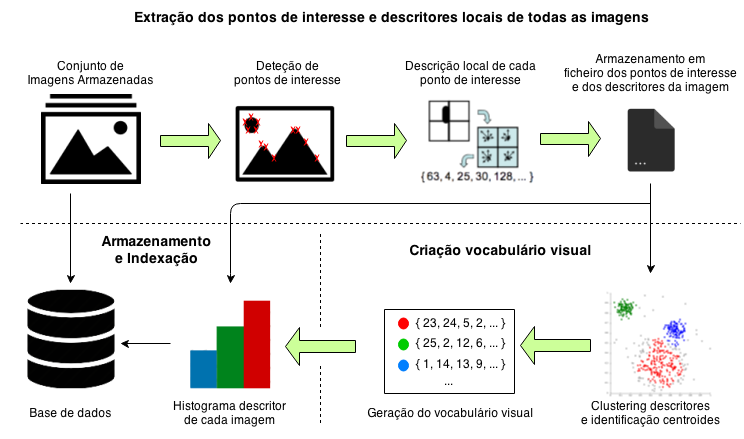
\includegraphics[width=0.95\linewidth]{./figures/infovisual}
\caption{Arquitetura do módulo de extração, processamento e armazenamento da informação visual. \textit{Adaptada de}~\cite{Bueno2011}}
\label{fig:infovisual}
\end{figure}

Como se pode ver pela figura~\ref{fig:infovisual} foram desenvolvidos três sub-módulos diferentes. O primeiro é o responsável pela extração dos descritores locais, o segundo utiliza o primeiro da gerar um vocabulário visual, e o terceiro e último sub-módulo utiliza os dois anteriores para armazenar um histograma descritor de cada imagem numa base de dados indexada a sua respetiva imagem. 
Em seguida é apresentada uma subsecção com a descrição para cada sub-módulo, como representado na figura~\ref{fig:infovisual}

\subsection{Extração dos pontos de interesse e descritores locais}

O primeiro passo no desenvolvimento deste módulo passou pela extração da informação visual. Esta informação visual deveria representar uma imagem eficientemente e de forma a possibilitar a criação de um vocabulário visual. Uma das formas possíveis e apresentadas na secção~\ref{sec:represent} é a utilização de um descritor local. Neste caso foi utilizado o descritor SIFT~\cite{Lowe1999, Lowe2004}, pois como referido na subsecção~\ref{subsubsec:surf}, apesar de ser mais lento e menos eficiente a mudanças de iluminação, este apresenta melhores resultados a variações de rotação, mudanças de escala e transformações na imagem. Para além disso, foi utilizada a ferramenta e biblioteca \textit{open source} VLFeat~\cite{vedaldi08vlfeat} que integra alguns dos algoritmos mais utilizados em visão computacional, e que inclui o algoritmo SIFT. Este, apesar de não possuir uma biblioteca para Python, permite a sua utilização através da linha de comandos.

Para o conjunto de imagens existentes foi necessário criar uma copia de cada imagem em escalas de cinzento e em formato \textit{.pgm} para ser utilizada pelo VLFeat. Utilizando assim estas imagens, o VLFeat armazena num ficheiro com o formato \textit{.sift} os pontos de interesse e os descritores de uma imagem, sendo necessário criar um ficheiro para cada imagem. Nesses ficheiros os dados são armazenados em formato ASCII. 
A informação armazenada apresenta-se da seguinte forma 

\begin{lstlisting}
318.861 7.48227 1.12001 1.68523 0 0 0 1 0 0 0 0 0 11 16 0 ...
318.861 7.48227 1.12001 2.99965 11 2 0 0 1 0 0 0 173 67 0 0 ...
54.2821 14.8586 0.895827 4.29821 60 46 0 0 0 0 0 0 99 42 0 0 ...
155.714 23.0575 1.10741 1.54095 6 0 0 0 150 11 0 0 150 18 2 1 ...
42.9729 24.2012 0.969313 4.68892 90 29 0 0 0 1 2 10 79 45 5 11 ...
229.037 23.7603 0.921754 1.48754 3 0 0 0 141 31 0 0 141 45 0 0 ...
232.362 24.0091 1.0578 1.65089 11 1 0 16 134 0 0 0 106 21 16 33 ...
201.256 25.5857 1.04879 2.01664 10 4 1 8 14 2 1 9 88 13 0 0 ...
... ...
\end{lstlisting}

onde cada linha contêm as coordenadas, escala e ângulo de rotação para cada ponto de interesse, nos primeiros 4 valores respetivamente, correspondendo os restantes ao vetor descritor de tamanho 128 como referido no capítulo~\ref{chap:estarte} na subsecção~\ref{subsubsec:sift}. Como o objetivo era utilizar as imagens originais, foram eliminadas as imagens temporárias com o formato \textit{.pgm}. O passo seguinte passou pelo desenvolvimento do submodelo responsável pela criação do vocabulário visual, que é apresentado na subsecção seguinte.

\subsection{Criação do vocabulário visual}

Este módulo é o responsável pela criação do vocabulário visual. Para a sua concretização foi necessário utilizar os ficheiros de extensão \textit{.sift} reproduzidos através da ferramenta VLFeat~\cite{vedaldi08vlfeat} no módulo anterior. Os passos seguintes basearam-se nos descritos em~\cite{Solem2012}. 

As palavras visuais não são nada mais do que um conjunto de vetores de características de imagens. Assim um vocabulário visual é o conjunto destas palavras visuais. Como todas as imagem possui muitos descritores locais, sendo que muitos podem ser semelhantes, é necessário agrupar todos os descritores de um conjunto de imagens e detetar aqueles que possam representar um conjunto de descritores semelhantes, e assim formar várias palavra visual, sendo uma palavra visual um centroide de um grupo.

Para criar um vocabulário visual foi então necessário utilizar um algoritmo de \textit{clustering} por partição, tendo sido escolhido o \textit{k-means} por ser um dos mais utilizados e eficiente, como foi referido no capítulo~\ref{chap:estarte} na secção~\ref{subsec:parti}. O algoritmo foi aplicado aos descritores de um conjunto de imagens aleatoriamente selecionadas. Como este algoritmo implica a pré definição do numero de \textit{clusters} (valor de \textit{k}), foi atribuído o valor 1000. Isto significa que são gerados 1000 \textit{clusters}, logo serão retornados 1000 centroides, o que significa que o nosso vocabulário visual possuirá 1000 palavras visuais.

% % talvez deva colocar aqui uma imagem

Para utilizar este vocabulário visual é necessário armazena-lo e indexar cada palavra visual a cada imagem. Assim o módulo é o responsável por este processo e é descrito de seguida.

\subsection{Armazenamento da informação visual}

\section{Matriz de distâncias entre imagens}